\chapter{Towards a New Architecture}
\label{chapter:towards-new-architecture}
The discussion in Chapter \ref{chapter:architecture} concluded with a proposal of a new future-proof architecture. We now present our implementation steps towards the new architecture with the implementation of a new user interface and the RESTful API.

\section{RESTful API}
As described in Chapter \ref{chapter:architecture}, communication between the user interface and the core of Tribler is facilitated by a RESTful API in our design. This Section explains the implementation details of the API in more detail.\\\\
The REST API has been implemented using facilities in the Twisted library. While there are plenty of Python solutions available that allow developers to create a web server in their application, we made the choice to use Twisted since it is already utilized to a great extent by Tribler. With the ability to integrate the REST API into the main application flow, we avoid having to create special constructions to execute the API on a separate thread like we are doing now with the video server. The API internally in Twisted is represented as a tree of resources which is in accordance with the REST architecture where the URL of the request can be treated like a path in the resource tree. If we visualize the import graph of the API package, this tree-like structure is somewhat visible, see Figure \ref{fig:importgraph-api}. We will highlight and discuss some important files in the API package:
\begin{itemize}
	\item \emph{rest\_manager.py}: this file contains the \emph{RESTManager} class which is responsible for starting and stopping the API. In addition, it  contains the \emph{RESTRequest} class which is a subclass of \emph{server.Request} (which in turn is instantiated by Twisted on an incoming request) and handles any exceptions that occurred during the serving of the HTTP request. Error handling in the API is discussed in Chapter \ref{subsec:error-handling-api}.
	\item \emph{root\_endpoint.py}: this file hosts the \emph{RootEndpoint} class which represents the root node of our resource tree. This class dispatches all incoming requests to the right sub nodes in the resource tree.
	\item \emph{util.py}: this file contains various helper functions, such as conversion utilities to easily transform channel and torrent data from the database into \emph{JavaScript Object Notation (JSON)} format that can be sent to the client that initiated a request.
\end{itemize}

\begin{figure}[h!]
	\centering
	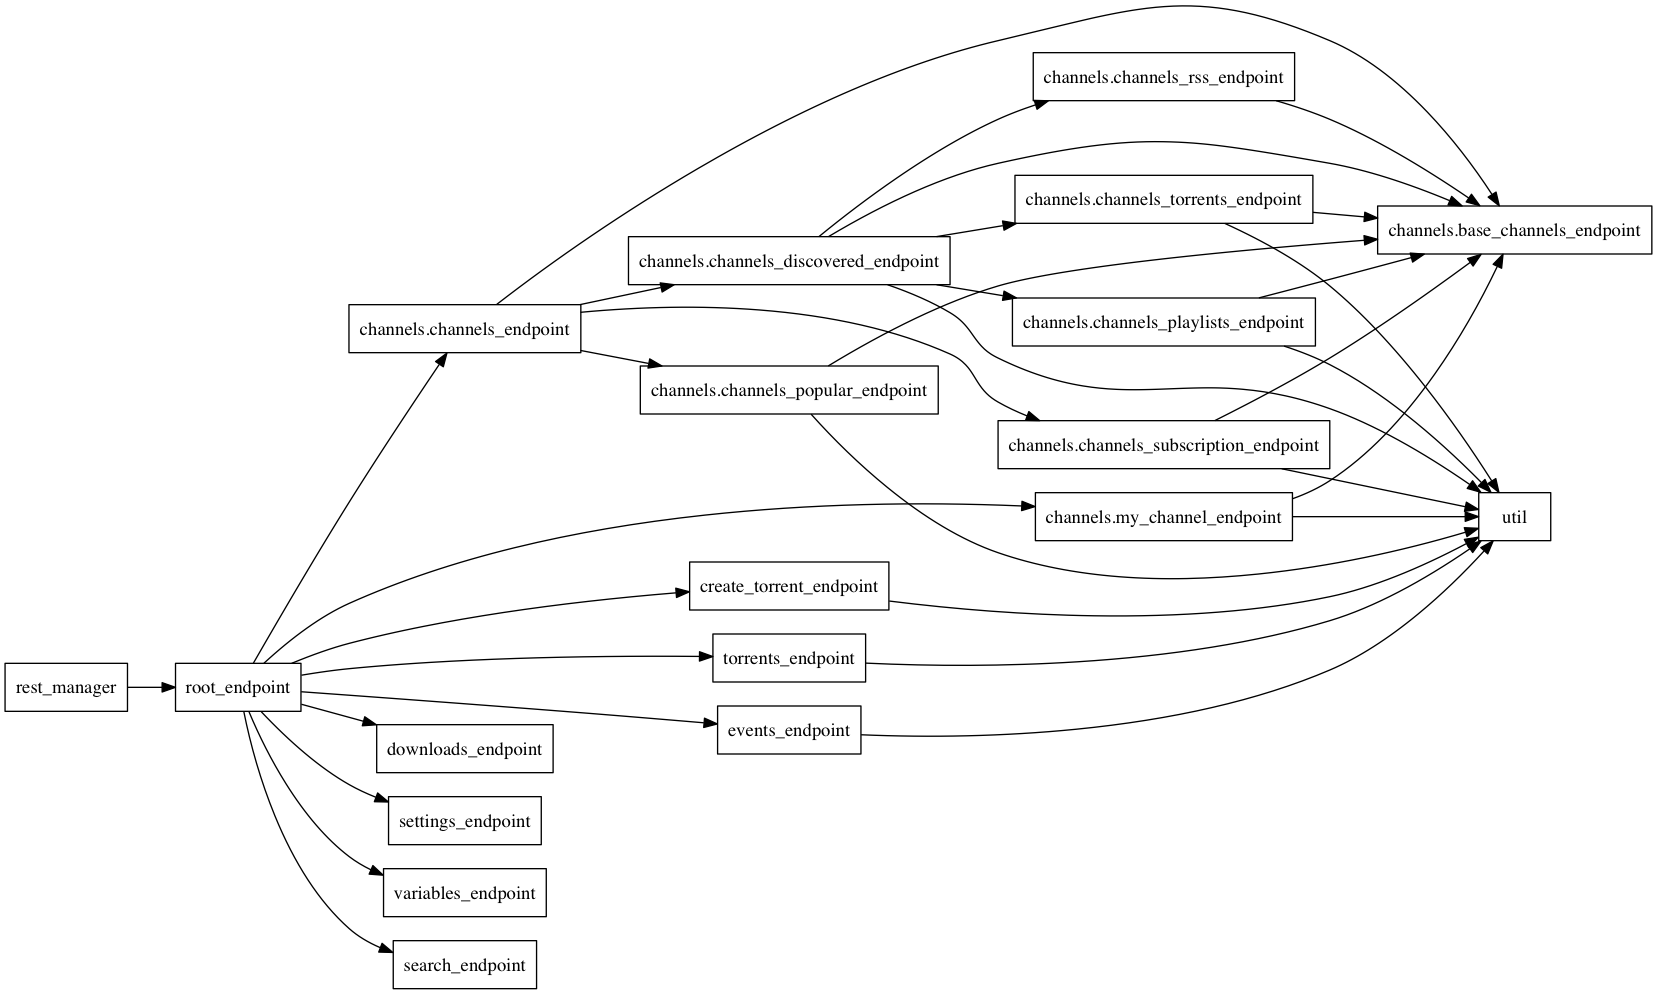
\includegraphics[width=1.0\columnwidth]{images/improving_qa/importgraph_api}
	\caption{The import graph of the REST API module.}
	\label{fig:importgraph-api}
\end{figure}

\subsection{Response Format}
Most data returned by the API is structured in JSON format. The JSON format is well adopted in the field of web engineering and easy to parse. However, in some occurrences we do not return JSON but instead, binary data. Examples of this are when exporting a torrent file where we return the content of the torrent file instead. While introducing some kind of inconsistency in the API, it allows for easier management of the response object since developers do not have to decode and parse the JSON object first.\\\\
Most of the endpoints are straightforward implementations where the client performs a request and some data is returned. There are situations where the client does a request and a asynchronous stream of data should be returned. For instance, this is the case when the user performs a search query. In some occurrences, data should be returned to the client, even if the client did not ask for this data. When a crash in the Tribler core code occurred, the client should be notified of this crash and possibly warn the user that he or she should restart the application. This motivates the design of an asynchronous events stream that notifies clients about interesting events in Tribler. This event stream has been implemented and all messages that are sent over the \emph{events} connection are shown in Table \ref{table:rest-api-events}. Developers can add new events with only a few lines of code.\\

\begin{table}
	\begin{tabularx}{\textwidth}{|l|X|}
		\hline
		\textbf{Event name} & \textbf{Description} \\ \hline
		\emph{events\_start} & The events connection is opened and the server is ready to send events.  \\ \hline
		\emph{search\_result\_channel} & Tribler received a channel search result (either remote or from the local database). The event contains the channel result data. \\ \hline
		\emph{search\_result\_torrent} & Tribler received a torrent search result (either remote or from the local database). The event contains the torrent result data. \\ \hline
		\emph{upgrader\_started} & The upgrade procedure in Tribler started. \\ \hline
		\emph{upgrader\_tick} & The status of the Tribler upgrader changed. This event contains a human-readable string with the status update, usable for display in a user interface. \\ \hline
		\emph{upgrader\_finished} & The Tribler upgrader finished. \\ \hline
		\emph{watch\_folder\_corrupt\_torrent} & The watch folder module has encountered a corrupt .torrent file. The emitted event contains the name of the corrupt file.\\ \hline
		\emph{new\_version\_available} & A new version of Tribler is available. The version number is part of the event.\\ \hline
		\emph{tribler\_started} & Tribler has completed the start up procedure and is ready to serve HTTP requests on all endpoints.\\ \hline
		\emph{channel\_discovered} & A new channel has been discovered. The events contains information about the discovered channel.\\ \hline
		\emph{torrent\_discovered} & A new torrent has been discovered. The events contains information about the discovered torrent.\\ \hline
	\end{tabularx}
	\caption{An overview of all events that are passed over the asynchronous events connection, part of the REST API.}
	\label{table:rest-api-events}
\end{table}

\subsection{Error Handling}
\label{subsec:error-handling-api}
A proper designed API should have a mechanism to notify users about any internal errors that occurred during requests. Our API returns HTTP response code 500 (\emph{internal server error}) when we observe a Python exception during a request. Moreover, we return a JSON-encoded response that contains more specific information about the caught exception such as the name of the exception, whether the error has been handled by the core and if available, the stack trace of the exception. An example of an error response is displayed in Listing \ref{lst:error-api-json}.

\begin{lstlisting}[caption={The response in JSON format returned when a Python exception is observed during the processing of an API request.},label={lst:error-api-json}]
{
  "error": {
    "message": "integer division or modulo by zero",
    "code": "ZeroDivisionError",
    "handled": false,
    "trace": [
        " File \"/Library/Python/2.7/site-packages/twisted/web/server.py\", 
        line 183, in process\n    self.render(resrc)\n", 
        ...
    ]
  }
}
\end{lstlisting}

\section{Graphical User Interface}
The amount of accumulated technical debt in the current graphical user interface of Tribler is devastating. After going through several development cycles where some impacting changes to the user interface have been made, the code base has reached the point where it might be more beneficial to design and implement a complete new user interface. 29,3\% of the Tribler code base, excluding Dispersy, is related to the user interface. We now will continue the discussion that has been initiated in Chapter \ref{chapter:problem-description} regarding the architecture of the user interface module. First, the structure of the current interface will be described. We will make the consideration between refactoring efforts of the existing user interface or creating and designing a new one. Additionally, encountered design decisions and implementation challenges are presented and discussed.

\subsection{Analysis of the Current GUI}
The user interface of the latest version of Tribler, 6.5.2, is unintuitive and cluttered with unused and unnecessary visual elements. There are various spelling errors in buttons and the navigation through the GUI is complex. The interface feels uncomfortable for users that are using Tribler for the first time and there are no instructions or guides for these users. For instance, when users are starting Tribler for the first time, there is no information provided about the content discovery process in the background. This is one of the improvements to the user interface we can consider to make.\\\\
When focussing on the code base, we notice that it is full of undesired workarounds and bad coding practices (code smells). Much functionality that should be located in the core module, is present in the code of the user interface package, including a relevance sorting algorithm of search results, code to manage important configuration settings and a large part of the start up procedure. There is no documented structure to be identified throughout the code and we can think of several reasons underlying that. One of these causes is the mindset of developers that the code base of the user interface is subordinate to the code related to core functionalities of Tribler: while it is often true that minor defects in the GUI are less critical than errors in important core functionalities such as the download engine, developer should always strive to write maintainable and well-designed code to prevent technical debt in the long term, a responsibility which is clearly neglected by user interface developers of Tribler. The fact that the GUI has undergone dramatic changes throughout ten years of research and development is an additional reason that led to this unstructured code base. Making short-term decisions were favoured over decisions that benefit the longer-term development process, leading to many code smells and huge amounts of technical debt.\\\\
By taking a closer look at the structure of the user interface code base, several files with many class definitions can be found. We already presented the import graph of the user interface code base in Figure \ref{fig:wx-import-graph} where we identified many cyclic dependencies. While cyclic dependencies are not always undesired at the granularity of a class file, we are dealing here with a web of dependencies between files, each file possibly consisting of multiple class definitions. Automated testing of individual classes has become significantly more involved with these dependencies.\\\\
We now turn our attention to the layout of user interface, where we use the wxPython inspection tool to investigate the widget structure of the interface at runtime. We noticed here that the naming convention of widget elements is unclear and does not represent content that the widget should present. For instance, the \emph{ActivityListItem} class is representing a list item in the left menu of Tribler, however, the name is confusing since the focus of this list item is not necessary a specific activity. We think that something along the lines of \emph{MenuListItem} would be a more appropriate name.\\\\
We noticed that the developers of user have attempted to reuse widget elements, especially noticeable in list-related widgets such as headers, footers and list row items. However, we think this should be classified as a failed attempt since the amount of flexibility is too much: by making widgets adapt to many different use-cases in the user interface, the complexity of the class definition increases significantly due to conditional code that is only executed in a subset of all the supported use-cases. We consider this an addition reason for the bad architecture as displayed in Figure \ref{fig:wx-import-graph}.\\\\
It is hard for developers to get familiar with the code base of the user interface and to modify it. We think the most appropriate metaphor of the user interface code base is a big ball of mud:

\begin{displayquote}
	\emph{A Big Ball of Mud is a haphazardly structured, sprawling, sloppy, duct-tape-and-baling-wire, spaghetti-code jungle. These systems show unmistakable signs of unregulated growth, and repeated, expedient repair. Information is shared promiscuously among distant elements of the system, often to the point where nearly all the important information becomes global or duplicated. The overall structure of the system may never have been well defined. If it was, it may have eroded beyond recognition. Programmers with a shred of architectural sensibility shun these quagmires. Only those who are unconcerned about architecture, and, perhaps, are comfortable with the inertia of the day-to-day chore of patching the holes in these failing dikes, are content to work on such systems.}\\
	- Brian Foote and Joseph Yoder, Big Ball of Mud\cite{foote1997big}.
\end{displayquote}

Due to the bad structure, huge amount of code smells and complexity of the code, we think that it is not worth the effort to refactor the code base of the current user interface and that it saves time to work on the design and implementation of a new user interface. However, we should think about a migration plan: while designing a new interface, critical issues should still be fixed in the current user interface code. By guaranteeing a minimal level of maintenance of the current GUI, we are not under time pressures to ship the new interface in a specific release of Tribler. Only when the new user interface is ready, stable and tested, we can remove the old interface.

\subsection{Choosing the Right Tools}
Before designing and implementing the new interface, we should first decide which library we would like to use. Because our proposed architecture in Figure \ref{fig:tribler7} is communicating to \emph{libtribler} using a RESTful API, this library does not necessary has to support the Python programming language. However, to make reuse of code easier and to maintain a consistent system which used the same programming language for all components, we will implement our new user interface in Python, There are plenty of libraries that are suitable. Below, several GUI libraries are summarized, together with a small description.
\begin{itemize}
	\item \emph{wxPython}\cite{rappin2006wxpython}: this is the current GUI library utilized in Tribler. \emph{wxPython} is built upon \emph{wxWidgets} and provides the Python bindings to this latter library. The library is cross-platform and one possibility is to use \emph{wxPython}. We already have a large code base written in \emph{wxPython} so continued usage of this library could allow us to reuse several widgets. The main disadvantages of this library are the minor inconsistencies across different platforms, the incompatible video player on MacOS and the lack of a visual designer, requiring us to specify the complete layout in Python code.
	\item \emph{Kivy}\cite{solis2015kivy}: the cross-platform library Kivy has been used in the past by Tribler developers, particularly in past attempts to run Tribler on Android\cite{de2014android}\cite{sabee2014tribler}. A decision to make use of the Kivy library for a new user interface enables us to reuse the interface logic already written for the Android app. The layout of Kivy can either be implemented using \emph{.kv} files or specified in code. While the library is rather new, it has gained significant attention and adoption in the Python community.
	\item \emph{Tkinter}\cite{lundh1999introduction}: the \emph{Tkinter} library is built upon the Tcl/Tk framework and is considered the de-facto GUI library for Python. Like wxPython, Tkinter does not provide a visual designer. The library is built-in in Python which means that no additional libraries have to be installed in order to start writing code. \emph{Tkinder} however is considered more suitable for simple applications due to the simplistic nature of the library.
	\item \emph{PyQt}\cite{summerfield2007rapid}: \emph{PyQt} provides the Python bindings for the Qt framework and is widely used in open-source and commercial applications. With a first version released in 1995, the Qt framework has evolved into a mature, well-maintained state. The library has a large documentation base and provides many different plugins to support a wide range of applications. One of these plugins is a visual WYSIWYG designer where the layout of an interface can be specified in a drag-and-drop manner. This generates a \emph{xml} file which can be read and parsed by \emph{Qt}. Visual styles can be specified using the \emph{Cascading Style Sheet} (CSS) language, widely used when styling websites.
\end{itemize}
Since the GUI will be an important aspect of Tribler, we wish to use a library that is mature, future-proof, well-maintained, easy to use and offers a large amount of tools so we can reduce the SLOC count that has to be maintained. We think that in the context of this thesis, choosing \emph{PyQt} is the best choice to build a new user interface. The fact that we can specify our layout using a visual editor is an enormous advantage since this will mean that we have less code to maintain. In addition, this allows other developers that are not familiar with the Tribler code base to contribute to the GUI. The \emph{Qt} visual designer also offers abilities for internationalization and translation of the user interface in multiple languages. Tasks like these are perfect opportunities for contributions in an open source project and can attract new developers. A screenshot of the visual designer in Qt is visible in Figure \ref{fig:qt-visualizer}.

\subsection{Designing the New GUI}
Designing a user-friendly interface is a non-trivial task and creating a proper design together with mock-ups, is a thesis task itself. Since the design of the new user interface is important but should not be the main focus of this work, we decide to adopt various design principles of existing applications that contain somewhat similar use-cases of Tribler.\\\\
In 2008, two design studies have been conducted on the Tribler GUI by master students\cite{triblerusabilityc2}\cite{triblerusabilityc4}. These studies have shown the Tribler user interface contains various inconsistencies and lack of visual feedback. Various users reported frustration because of features that did not function as they expected. This is a common phenomena when designing a user interface as a developer: developers tend to assume that users understand concepts integrated in the user interface, such as torrents, channels while this is often not the case. In fact, it is beneficial to have to user interface designed by a specialist, however, this is not possible due to lack of manpower and budget.\\\\
Most applications that provide torrent download capabilities have a similar interface: they present a list with downloads and a detail window with specific information about a selected downloads. The old user interface also follows this design when displaying the downloads and we see no reason for now to make significant changes to this. However, Tribler provides more abilities than downloading torrents: browsing through content and managing channels are also use-cases that should be taken into consideration.\\\\
We believe that YouTube\footnote{https://youtube.com} is an example of application that has a large feature overlap with Tribler, namely the browsing and streaming of videos, managing channels and creating playlists. The home page of the YouTube interface is visible in Figure \ref{fig:youtube-interface}. We copy the left menu as present in the current interface and use it in the new GUI, however, we modify it slightly: first, we add an option to open and close the menu by clicking the hamburger menu in the upper-left corner since the menu might clutter the interface and does not always need to be visible. Next, we make use of icons so users can faster identify what the idea behind each menu option is. In general, we are using more icons in the new user interface since we believe that the old GUI contains too textual elements.\\\\
To make the user interface more appealing and less boring, we attach a thumbnail to each content item. There is however an issue here: the thumbnails as implemented in the current system are not working correctly. Since the implementation of a new thumbnail mechanism is outside the scope of this thesis, we use thumbnails that are generated based on the content. This is a technique also adopted by popular platforms such as Stack Overflow and Telegram to display a profile image when the user has not uploaded a picture yet.\\\\
Finally, we want to get rid of buttons that are only appearing when hovering over content like currently implemented in the old GUI. To make it more clear that a specific action can be performed with content, we do not conditionally hide and show buttons but instead, persistently display these widgets.\\\\
Due to time constraints, it is decided to not implement all features available in the old interface. Functionalities such as the debug panel, local content filtering and sorting of content will not be implemented in the first iteration of the new user interface. The focus of this new interface will be centred around searching and streaming content.\\\\
Our vision during development of this interface is that in essence, it should only display data and do as few processing operations on this data as possible. This means that various code that is now present in the user interface library should be moved to the Tribler core, such as the search results ranking algorithm.

\begin{figure}[t]
	\centering
	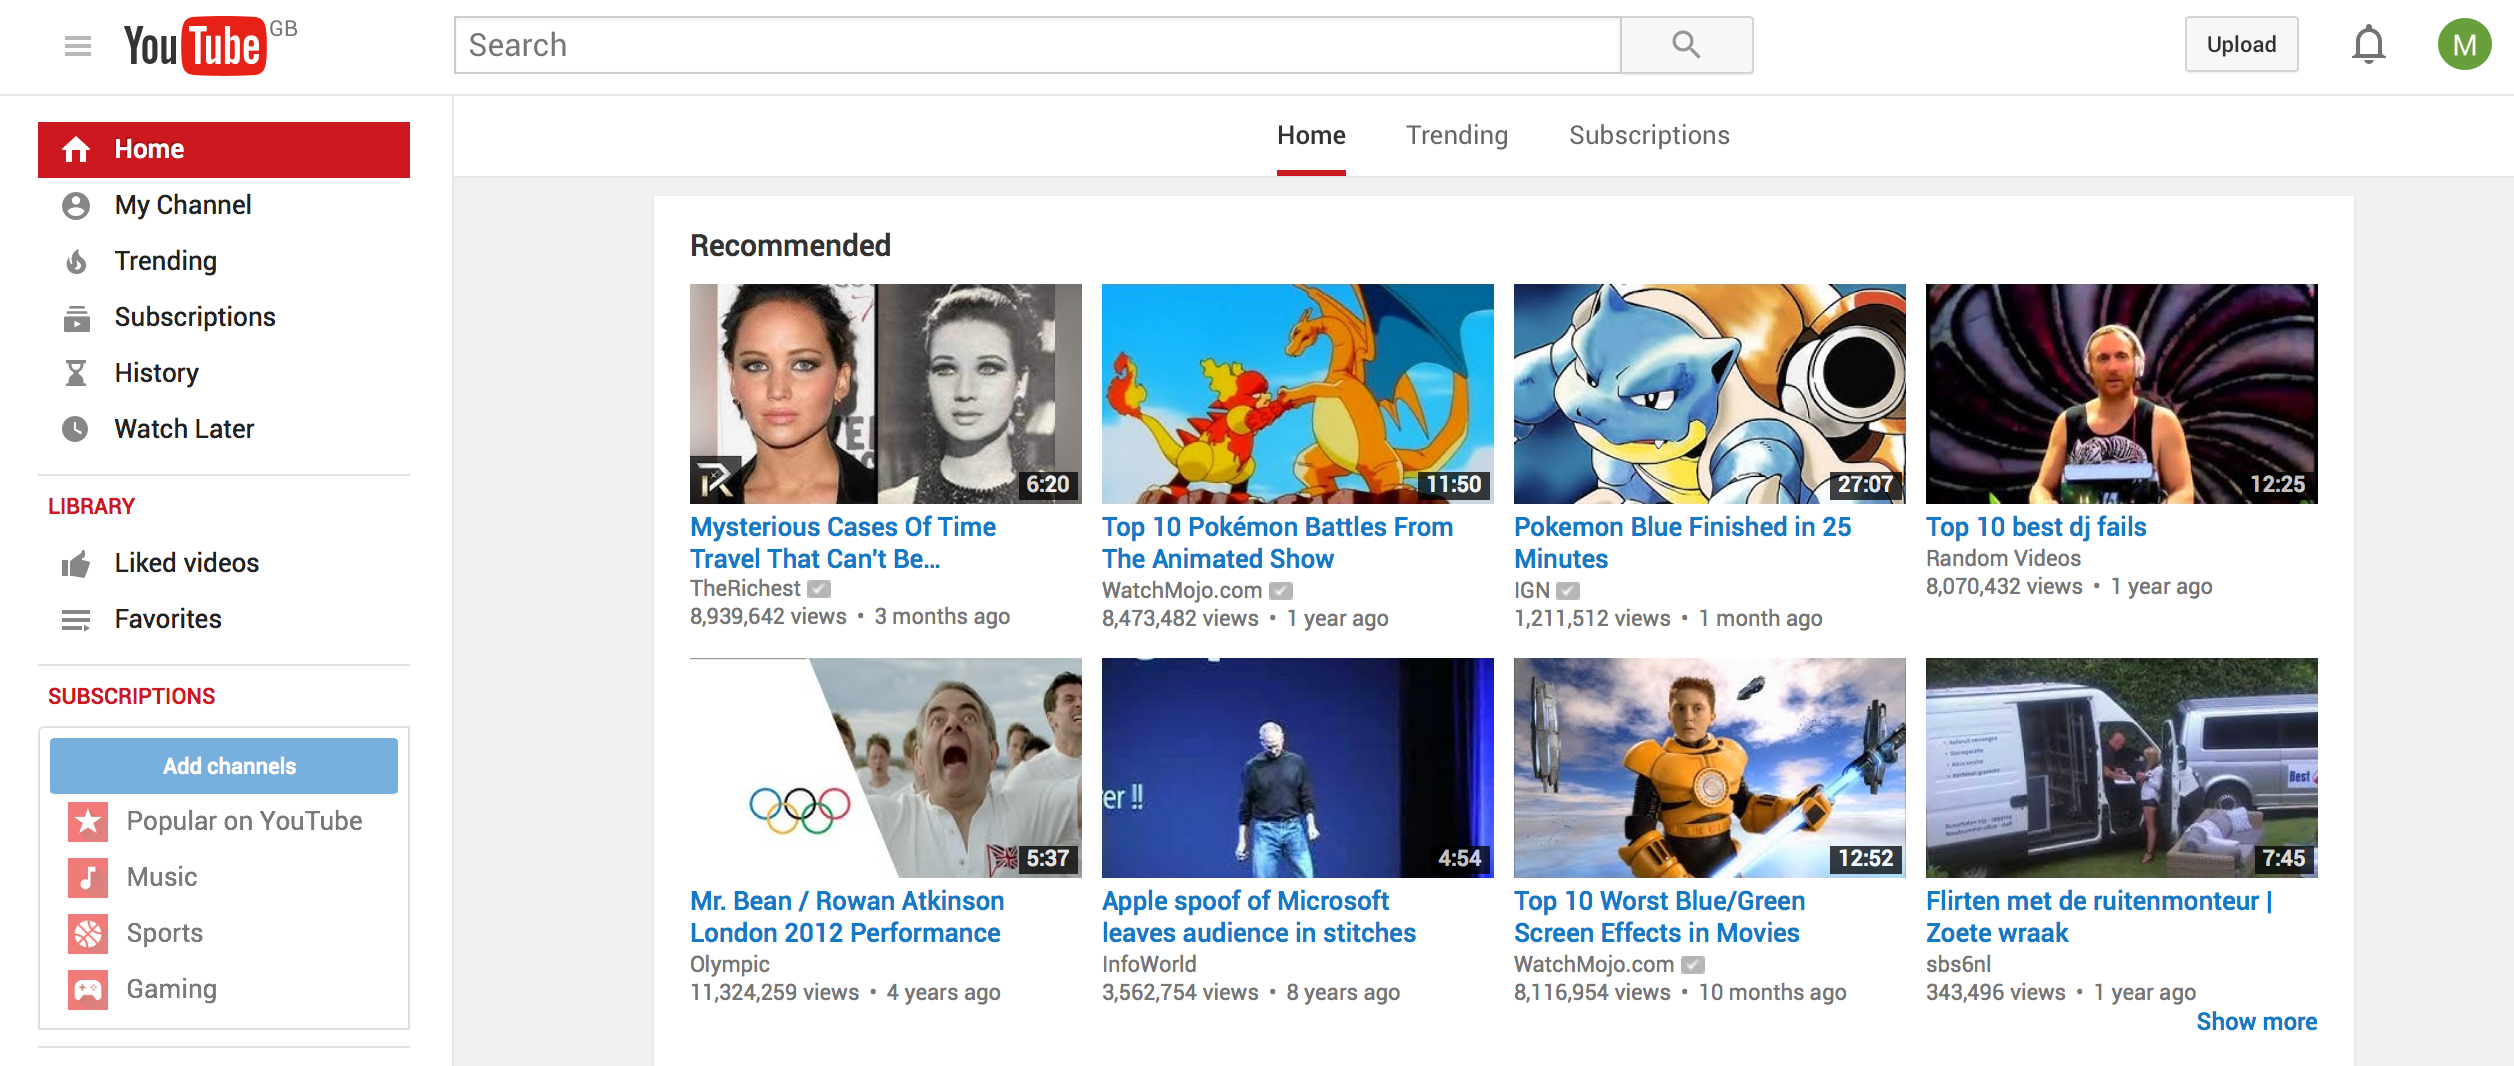
\includegraphics[width=1.0\columnwidth]{images/implementation/youtube_interface}
	\caption{The user interface of YouTube.}
	\label{fig:youtube-interface}
\end{figure}

\subsection{Implementing the GUI}
The result after implementation of the new GUI is visible in Figure \ref{fig:new-gui-1}. The majority of the new user interface has been built using the visual designer, part of \emph{Qt}. The Python code that we had to write is responsible for handling requests to the Tribler core, displaying the right content in lists and to manage interface-related settings.\\

\begin{figure}[t]
	\centering
	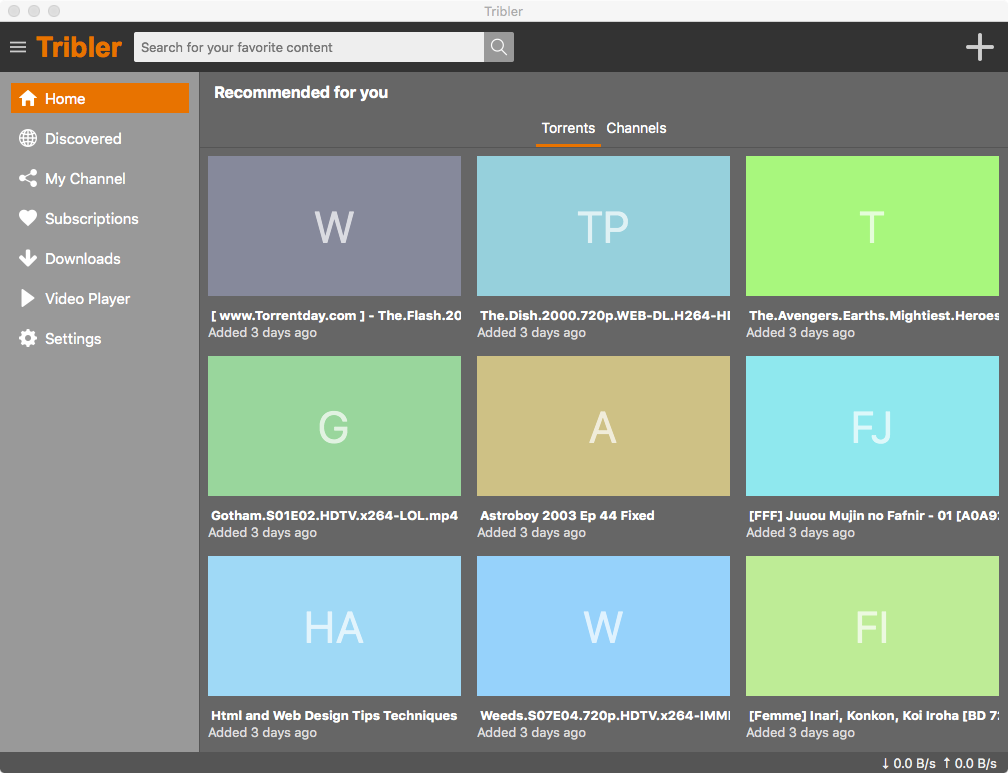
\includegraphics[width=1.0\columnwidth]{images/improving_qa/newgui1}
	\caption{The home page of the new Tribler GUI.}
	\label{fig:new-gui-1}
\end{figure}

A key feature of the \emph{Qt} library is the signal-slot mechanism which facilitates communication between code and widgets. Widgets in \emph{Qt} can contain signals, events they want to broadcast. Some widgets have built-in signals, for instance, a button emits a \emph{clicked} signal if the user clicks on this widget with the mouse. Other widgets or objects in Python can subscribe to these signals and perform specific actions when the signal is observed. Signals and slots can either be created using code, or designed in the visual designer. To keep the amount of written code to a minimum, we decided to specify our widgets connections in the visual designer as much as possible.\\\\
During development of the user interface, we encountered various interesting implementation challenges that required some form of analysis. We will now present these issues and discuss them.

\subsubsection{\textbf{Scalability of List Items}}
The \emph{Qt} framework allows to display potentially many items in a simple list. The performance decreases dramatically if custom widgets are rendered in a list. Loading 1.000 of such list items takes over 22 seconds on a high-end iMac computer which is an unacceptable amount of latency when displaying a list with content. For each item in the list, the associated interface definition file has to be read, parsed and rendered, possibly many times per second. Channels hold potentially several thousand of torrents which should be presented in the GUI in a timely matter.\\\\
This scalability bottleneck has been solved by utilizing a simple technique: lazy loading. By taking advantage of a lazy loading approach where additional data is loaded in chunks (30 items in our new interface) when the user has scrolled to the end of a list, we can postpone and possibly avoid loading the whole list at once. This solution has also been implemented in the old user interface. By loading only a subset of the list rows, the user experience can be significantly increased since users don't have to wait until the whole list of items is loaded, at the cost of a small delay when the end of the list is reached. The implementation of this lazy-loading solution is general enough to be reused for any type of list in Qt and is located in the \emph{lazyloadlist.py} source file. This implementation however, still resulted in a significant period of waiting when the next set of items is being loaded, around one second. It turned out that loading and parsing of the interface definition file is a time-consuming operation. The solution to reduce this processing time is to pre-load the interface definition as soon the user interface starts. This has a minor effect on the total start-up time (around 40 milliseconds on a high-end iMac device). This the latency when loading additional items to several hundred milliseconds.

\subsubsection{\textbf{A Functioning Multi-platform Video Player}}
One of our main focusses of the new GUI is the streaming of videos. The embedded video player in the old user interface did not function correctly on MacOS due to incompatibilities with the wxPython library. The video player has been implemented using the popular VLC library\cite{vlcwebsite}, a free and open source cross-platform multimedia player and framework that plays most media files. We started the design of the new GUI by creating a prototype where the implementation of a cross-platform, embedded video player with support for starting and stopping a video is centrally involved. While example code was available for the PyQt4 library using VLC bindings, there were some minor quirks when implementing the video player using PyQt5, mostly involved around obtaining a reference to the frame of the video player (which should be done in different ways on each platform). The code for this prototype player has been used as basis for the implementation of the video player in the new user interface of Tribler and is available as open-source project on GitHub\cite{vos2016vlc}.

\section{Threading Model Improvements}
In Section \ref{subsec:architecture-twisted}, we discussed that the current threading model is complex and prone to implementation errors introduced by developers. The implementation of a new GUI and a RESTful API as described in the last sections, has led to a cleaner and stable threading model. Now that the user interface runs in a separate, dedicated process and thanks to the removal of \emph{wxPython} from Tribler, we are now able to run the Twisted reactor on the main thread. This enables us to get rid of the confusing decorators to switch between the main and reactor thread since from now on, we only have one thread (besides the threadpool) to schedule calls on. Getting rid of the abundant thread switching should increase performance since we avoid overhead introduced by the context switches. The new, simplified threading model is presented in Figure \ref{fig:new-threading-model}.

\begin{figure}[h!]
	\centering
	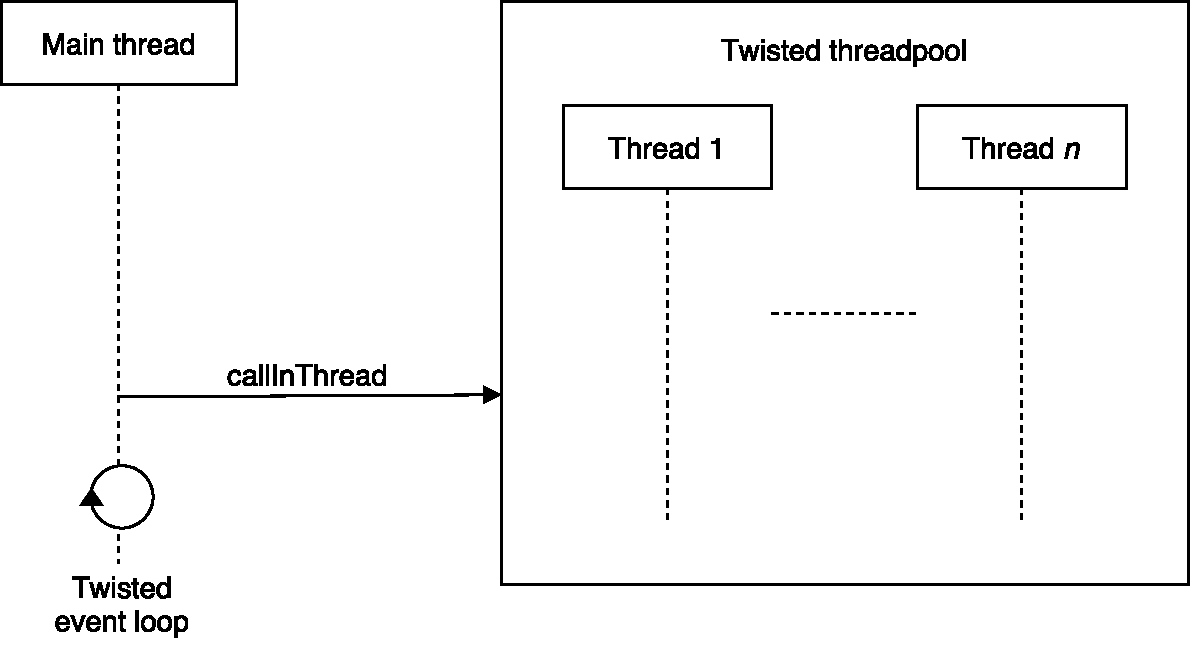
\includegraphics[width=0.7\columnwidth]{images/improving_qa/new_threading_model_tribler}
	\caption{The new, simplified threading model in Tribler 7, together with the primitives to schedule operations on the threadpool.}
	\label{fig:new-threading-model}
\end{figure}

\section{Relevance Ranking Algorithm}
\label{sec:relevance-ranking-algorithm}
We significantly improved the search algorithm in Tribler by adjusting the search result sorting mechanism. When users are performing a keyword search in the user interface, the returned search results are sorted according to a relevance ranking algorithm that considers several attributes of the search results. A key problem of this algorithm is that the implementation is located inside the user interface code base. Essentially, sorting search results should be considered a task where the Tribler core is responsible for. Moving the algorithm to the core module seems to be a adequate solution but this requires us to understand the old relevance ranking rules so we can reimplement the algorithm in the core module. Unfortunately, the code that is responsible for the relevance ranking is hard to read and understand. Even worse, it lacks proper documentation, making the functioning algorithm rather obscure. Moreover, the code it split between several classes, making it though to understand its behaviour\todo{review}.

\subsection{Old Ranking Algorithm}
Channels and torrents are sorted according to different criteria: channels are ranked on the number of torrents where ones that have a higher number of torrents, are displayed at a higher position in the list. The algorithm to sort torrents on relevance is more involved and uses five different scores. These scores are determined as follows (ordered on importance):
\begin{enumerate}
	\item The number of matching keywords in the name of the torrent. Keywords are determined by splitting the name of a torrent on non-alphabetical characters. Common keywords such as \emph{the} or \emph{be} are filtered out and not considered as a keyword.
	\item The position of the lowest matching keyword in the torrent name. For instance, when searching for \emph{one} and there is a torrent result named \emph{Pioneer-one-S01E03.avi}, the position of the lowest matching keyword is 2, since \emph{Pioneer} is not present in the search query.
	\item The number of matching keywords in the file names that the torrent contains.
	\item The number of matching keywords in the extension of the files this torrent contains (for instance, \emph{avi}, \emph{iso} etc).
	\item A sub score that is based on several (normalised) attributes of the torrent. This sub score is determined after the set of local search results are constructed. To calculate this sub score, the following formula is used: 
	
	\begin{equation}
	\label{eq:score-old-ranking-5}
	s = 0.8n_s - 0.1n_{vn} + 0.1n_{vp}
	\end{equation}
	
	 where $ s $ is our sub score, $ n_s $ denotes the number of seeders (this will be 0 if this information is not available yet), $ n_{vn} $ the number of negatives votes of this torrent and $ n_{vp} $ the amount of positive votes this torrent has received. We should note that the number of positive and negative votes do not exist any more and as a consequence will always be zero, making this score only dependent on the number of seeders, which during our observation is often zero. The normalization process calculates the standard score for every data item, using the following formula:
	
	\begin{equation}
	\label{eq:normalization-standard-score}
	z = \frac{x - \mu}{\sigma}
	\end{equation}
	
	where $ z $ is our normalized score, $ x $ the score to be normalized, $ \mu $ the mean of the data set and $ \sigma $ the standard deviation of the data set.
	
\end{enumerate}
For each torrent, the set of five scores as described above is determined. The comparison between two torrents now proceeds based on these five determined scores, starting with the first score, proceeding to the next score in case when two scores are equal.\\\\
Finally, the list is prepared and a channel result is inserted between every five torrent items in the list. This is done since usually, the amount of torrents is much bigger than the amount of channels. Not only channels matching the search query are displayed: for each torrent, the most popular channel that contains this specific torrent, is determined and also considered in the list of results.\\\\
While the algorithm as described above takes many factors in consideration, we detected some problems and possible improvements:
\begin{itemize}
	\item One of the main problem is that the amount of matches inside a torrent name/torrent file name is not taken into consideration. For instance, when searching for \emph{Pioneer One}, a torrent named \emph{Pioneer One Collection} probably has a higher relevance than a torrent named \emph{Pioneer One - Episode 3, Season 4} since the matching in the first case is considered better.
	\item The relevance sorting of channels in the result set is only dependent on the number of torrents in that channel. The number of matching terms in the channel name and description is not even considered.
	\item When building the inverted index in the SQLite database for the full text search, duplicate words are removed. This means that when we search for \emph{years}, a torrent named \emph{best years} will be ranked equal to a torrent named \emph{years and years} (if we only consider a ranking based on the torrent name). However, the torrent named \emph{years and years} should be assigned a higher relevance since the keyword \emph{years} occurs twice in the latter example. Another example is when searching for \emph{iso}. A torrent file that contains 100 \emph{iso} files is currently ranked equivalent to a torrent file that only has one \emph{iso} file.
	\item The current relevance ranking algorithm only returns results that matches all given keywords. So when searching for \emph{pirate audio}, only torrents are returned that are matching on both terms. It might be better to show the user also torrents matching 'pirate' and matching 'audio' (while still giving a higher relevance score to torrents that matches 'pirate audio').
	\item The ranking of search results are dependent on each other. This is noticeable when calculating the score based on normalized data. To normalize this data, we should have information about other search results. This prevents a "streaming-like" search operation where the relevance score of each search item is only dependent on data that search item contains and no other data.
\end{itemize}

\subsection{Designing a New Ranking Algorithm}
In the previous Subsection, we described the old ranking algorithm, together with some problems and improvements. In this Subsection, we will design a new, robust and simplified algorithm. The heart of the algorithm will be based on Okapi BM25, a ranking function used by search engines to rank matching documents according to their relevance to a given search query\cite{jones2000probabilistic}. BM25 can be implemented using the following formula:

\begin{equation}
\label{eq:bm25}
s = \sum_{i=1}^{n} IDF(q_i) \frac{f(q_i, D)(k_1 + 1)}{f(q_i, D) + k_1 (1 - b + b * \frac{|D|}{avgdl})}
\end{equation}

In the formula above, we have a document $ D $ where the length of $ D $ is denoted as $ |D| $. There are $ n $ keywords present in our search query, $ q_i $ representing the keyword at index $ i $. $ f(\cdot, D) $ gives the frequency of keyword $ q_i $ in document $ D $. The $ IDF(q_i) $ denotes the \emph{inversed document frequency} of keyword $ q_i $ which basically states how important a keyword is in a document. The IDF is usually calculated as:

\begin{equation}
\label{eq:bm25-idf}
IDF(q_i) = log\frac{N - n(q_i) + 0.5}{n(q_i) + 0.5}
\end{equation}

where $ N $ is the total number of documents and $ n(q_i) $ is the number of documents containing keyword $ q_i $. The full text search engine in SQLite offers tools to easily calculate a BM25 score when performing a query. Unfortunately, this is not implemented in the engine we are currently using, FTS3. This motivates us to upgrade to a newer engine, FTS4, which offers the necessary tools to easily calculate the BM25 score. This requires a one-time upgrade of the database engine of users which should be performed when Tribler starts.\\\\
Each search result is assigned a relevance score. The final relevance score assigned to a torrent is dependent on three other sub-scores that are calculated using the BM25 algorithm and is a weighted average of the sub-scores, determined by the name of the torrent (80\%), the file names of the torrent (10\%) and the file extensions of the torrent (10\%). The final relevance score of a channel is the weighted average of the BM25 score of the name of the channel (80\%) and the description of the channel (20\%).\\\\
While this works well when searching for local search results, we should also be able to assign a relevance rank to incoming remote torrent or channel results. To do this, we keep track of the latest local searches and the gathered information that is used by Equations \ref{eq:bm25} and \ref{eq:bm25-idf}. If we receive an incoming search result, we are using that stored information to quickly determine the relevance score of the remote result. Using this approach, we avoid a lookup in the database for every incoming remote search result. If we have no information about the latest local database lookup available, we assign a relevance score of 0 to the remote result.

\subsection{Ranking in the User Interface}
After each search result got a relevance score assigned, we should order the search results in the user interface. We cannot make the assumption that the data we receive from Tribler is already sorted (however, a relevance score should be available) thus we need a way to insert items dynamically in the list. The lazy-loading list we are using in the user interface makes this task more difficult since we both have to insert items dynamically in the list and make sure that we are not rendering too much row widgets. We also wish to avoid reordering operations as they are computational expensive to perform.\\\\
The implemented solution works as follows: in the user interface, we maintain two lists in memory: one list that contains the torrent search results and another list that contains channel search results. We guarantee that these lists are always sorted on relevance score. Insert operations in this list are performed using a binary search to determine the new position of the item in the sorted list, leading to a complexity of $ O(log\ n) $ for each insert operation (where $ n $ is the number of items in the list). In the visible result list, we first display channels, which are usually only a few. The rationale behind this idea is that users prefer to see matching channels since these channels might contain many relevant torrents. This solution is scalable to many search results.\\\\
A presentation of the performance of the new relevance ranking algorithm is presented in Chapter \ref{sec:local-content-search}.

\begin{figure}[h!]
	\centering
	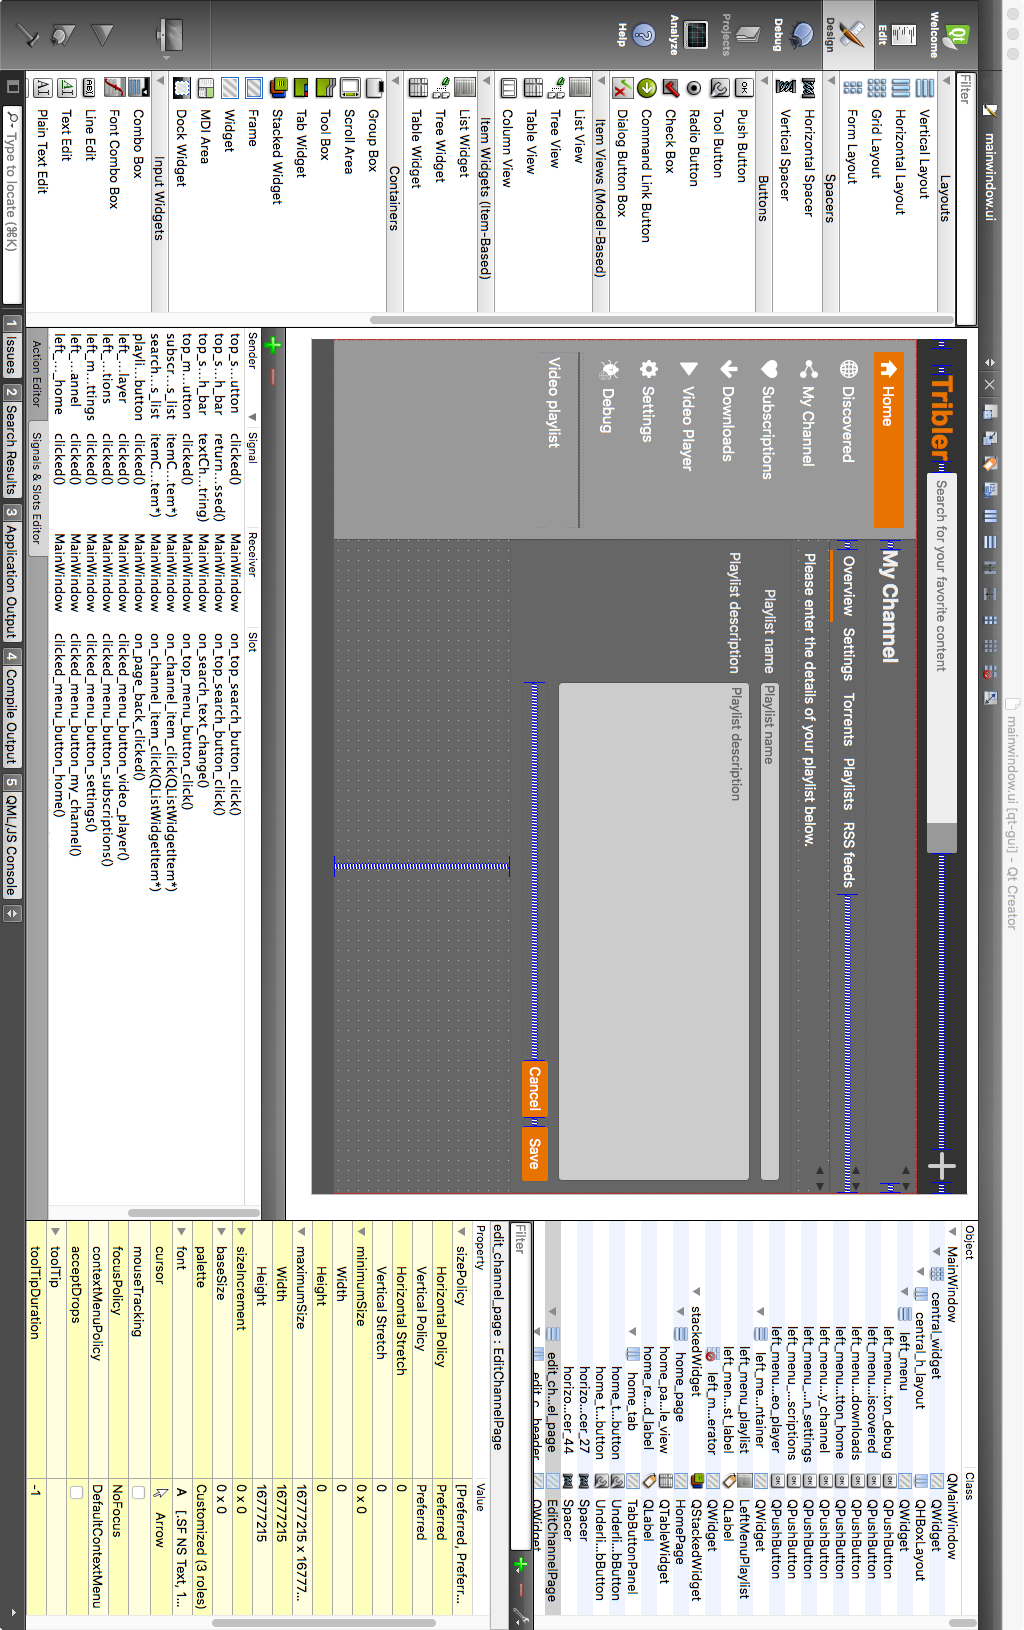
\includegraphics[width=1.0\columnwidth]{images/improving_qa/qt_designer}
	\caption{The Qt visualizer tool used to create the new user interface of Tribler.}
	\label{fig:qt-visualizer}
\end{figure}